\documentclass[11pt]{article}
\usepackage[margin=1in]{geometry}
\usepackage[T1]{fontenc}
\usepackage{lmodern}
\usepackage{amsmath,amssymb}
\usepackage{graphicx}
\usepackage{booktabs}
\usepackage{xcolor}
\usepackage[hidelinks]{hyperref}
\usepackage[numbers,sort&compress]{natbib}
\usepackage{microtype}
\usepackage{caption}
\graphicspath{{figures/}}
\captionsetup{font=small,labelfont=bf}
\newcommand{\nPTrExp}{466}
\newcommand{\nPTrPos}{106}
\newcommand{\nPTrWeeks}{201}
\newcommand{\nPTrScored}{83}
\newcommand{\nPTrScoredExp}{253}
\newcommand{\nPTrMedian}{2}
\newcommand{\nPTrRate}{23}
\newcommand{\nPVaExp}{672}
\newcommand{\nPVaPos}{113}
\newcommand{\nPVaWeeks}{105}
\newcommand{\nPVaScored}{56}
\newcommand{\nPVaScoredExp}{439}
\newcommand{\nPVaMedian}{6.5}
\newcommand{\nPVaRate}{17}
\newcommand{\nPTeExp}{393}
\newcommand{\nPTePos}{36}
\newcommand{\nPTeWeeks}{86}
\newcommand{\nPTeScored}{30}
\newcommand{\nPTeScoredExp}{179}
\newcommand{\nPTeMedian}{5}
\newcommand{\nPTeRate}{9}
\newcommand{\nSTrExp}{776}
\newcommand{\nSTrPos}{140}
\newcommand{\nSTrWeeks}{229}
\newcommand{\nSTrScored}{100}
\newcommand{\nSTrScoredExp}{443}
\newcommand{\nSTrMedian}{4}
\newcommand{\nSTrRate}{18}
\newcommand{\nSVaExp}{905}
\newcommand{\nSVaPos}{134}
\newcommand{\nSVaWeeks}{105}
\newcommand{\nSVaScored}{63}
\newcommand{\nSVaScoredExp}{601}
\newcommand{\nSVaMedian}{8}
\newcommand{\nSVaRate}{15}
\newcommand{\nSTeExp}{738}
\newcommand{\nSTePos}{52}
\newcommand{\nSTeWeeks}{89}
\newcommand{\nSTeScored}{39}
\newcommand{\nSTeScoredExp}{383}
\newcommand{\nSTeMedian}{9}
\newcommand{\nSTeRate}{7}
\newcommand{\qwenAutoPct}{10}
\newcommand{\gemmaAutoPct}{34.9}
\newcommand{\aucPrimaryTest}{0.671}
\newcommand{\aucSecondaryTest}{0.751}


\title{Engineering Serendipity in Personal Agents:\\
A Pre-registered Fifteen-Year Single-Subject Test of\\ Exploitation versus Exploration}
\author{Carl Kho\\ \small Independent researcher}
\date{September 2026}

\begin{document}
\maketitle

\begin{abstract}
A personal agent trained on a person's own history can learn to answer ``what would I do?''. An agent meant to augment that person must also ask ``what am I failing to consider?''. We test whether the two come apart on one subject's fifteen-year record of 3.08 million messages across nine platforms. The task is retrospective ranking of weak-tie inbound exposures (the first message in a thread, or one that revives a thread silent for six months), each labelled by whether the thread was still active a year later after at least five further separate exchanges. Features use only information available at exposure time; message semantics come from typed judgments by local language models. After developing the method on earlier years, we pre-registered the analysis and opened the 2024 to 2025 test period once. A ranker trained to predict which messages the subject would answer placed the exposures that became lasting ties below random order (difference in mean reciprocal rank $-0.14$, 95\% CI $[-0.20, -0.07]$). A hybrid exploration score did worse than random exploration with an equal diversity budget ($-0.22$, $[-0.27, -0.16]$); validation tuning had given its uncertainty and information-gain terms zero weight, leaving relevance, novelty, a judged option value and a cost penalty. Ranking new threads first was not better than the random baseline. Ties that lasted tended to begin as casual personal messages rather than invitations or organizational outreach, and two independent local judges agree. Separately, a personal LoRA adapter partly predicts the subject's next action (37.8\% versus 28.0\% top-1 in a five-way choice). In this record, no exploration score we tried beat random exploration with coverage on mean reciprocal rank. Code and pre-registration are public; the data are not.
\end{abstract}

\section{Introduction}

People who record large parts of their lives accumulate something unusual: a long, dense trajectory of one agent acting in the world. The obvious use of such a record is imitation. Given enough of a person's history, a model can learn to predict what they will do next, and a personal agent built on that model can act in their style. Behavioral cloning of this kind is well understood \citep{pomerleau1991efficient,ross2011reduction}, and we report below that it works to a measurable degree on the subject of this study.

Imitation has a known failure mode that matters more for a personal agent than for a robot. A good clone reproduces its source's policy, including the parts of that policy the person would change if they could see the alternatives. A recommender trained on a person's engagement learns what they already attend to and serves more of it, which is the feedback loop studied in recommender systems as algorithmic confounding and homogenization \citep{chaney2018algorithmic}. The subject of this study noticed that several consequential turns in his own life began with exposures his contemporaneous preferences would likely have ranked low: an unsolicited message, a stranger's invitation, an unfamiliar community. If that is common, an agent that optimizes for what the subject would engage with would filter out exactly those events.

Reinforcement learning has a vocabulary for this tension. Exploitation chooses the action with the highest estimated value. Exploration spends some budget on actions whose value is uncertain, because the estimate may be wrong and because trying them reveals information \citep{auer2002finite,russo2018tutorial}. Curiosity, information gain and empowerment formalize why an agent might prefer the unfamiliar \citep{schmidhuber2010formal,houlsby2011bayesian,pathak2017curiosity,klyubin2005empowerment}. The recent argument that agents should learn primarily from their own streams of experience \citep{silver2025era} makes the question concrete for personal agents: if the stream is one human life, what should the agent explore on that person's behalf?

This paper asks the narrowest testable version of that question. Given the subject's logged history up to a moment, and the set of people who reached out to him that week, does a ranker built to predict his engagement surface the exposures that later became lasting ties? Can exploration terms of the kind the literature proposes do better at the same budget? We study one person over fifteen years, using only what was logged, with outcomes defined in advance and a test period we opened once.

\paragraph{Contributions.}
\begin{enumerate}
\item A leakage-controlled retrospective benchmark for engineered serendipity on one subject: 35{,}168 inbound contact events from 2011 to 2026, of which 3{,}719 are weak-tie exposures and 3{,}221 have complete one-year outcomes computed automatically.
\item A pre-registered test on held-out years (2024 to 2025). A relevance ranker buries later-lasting ties (supported). A hybrid exploration score does not beat random exploration with an equal diversity budget (rejected). New-thread-first ranking is inconclusive.
\item Evidence from typed judgments by two local language models that the exposures which became lasting ties were more often personal chat and less often invitations or organizational outreach, the messages an opportunity-seeking agent would prioritize.
\item A recomputation of a prior behavioral-cloning result on the same subject from its raw per-case scores, and an explicit account of what the data cannot yet support. In particular, the platform-recommendation ``mirror'' channel we propose cannot be tested, because platforms export their recommendations only as present-day snapshots.
\end{enumerate}

\section{Problem setting}
\label{sec:setting}

\begin{figure}[t]
\centering
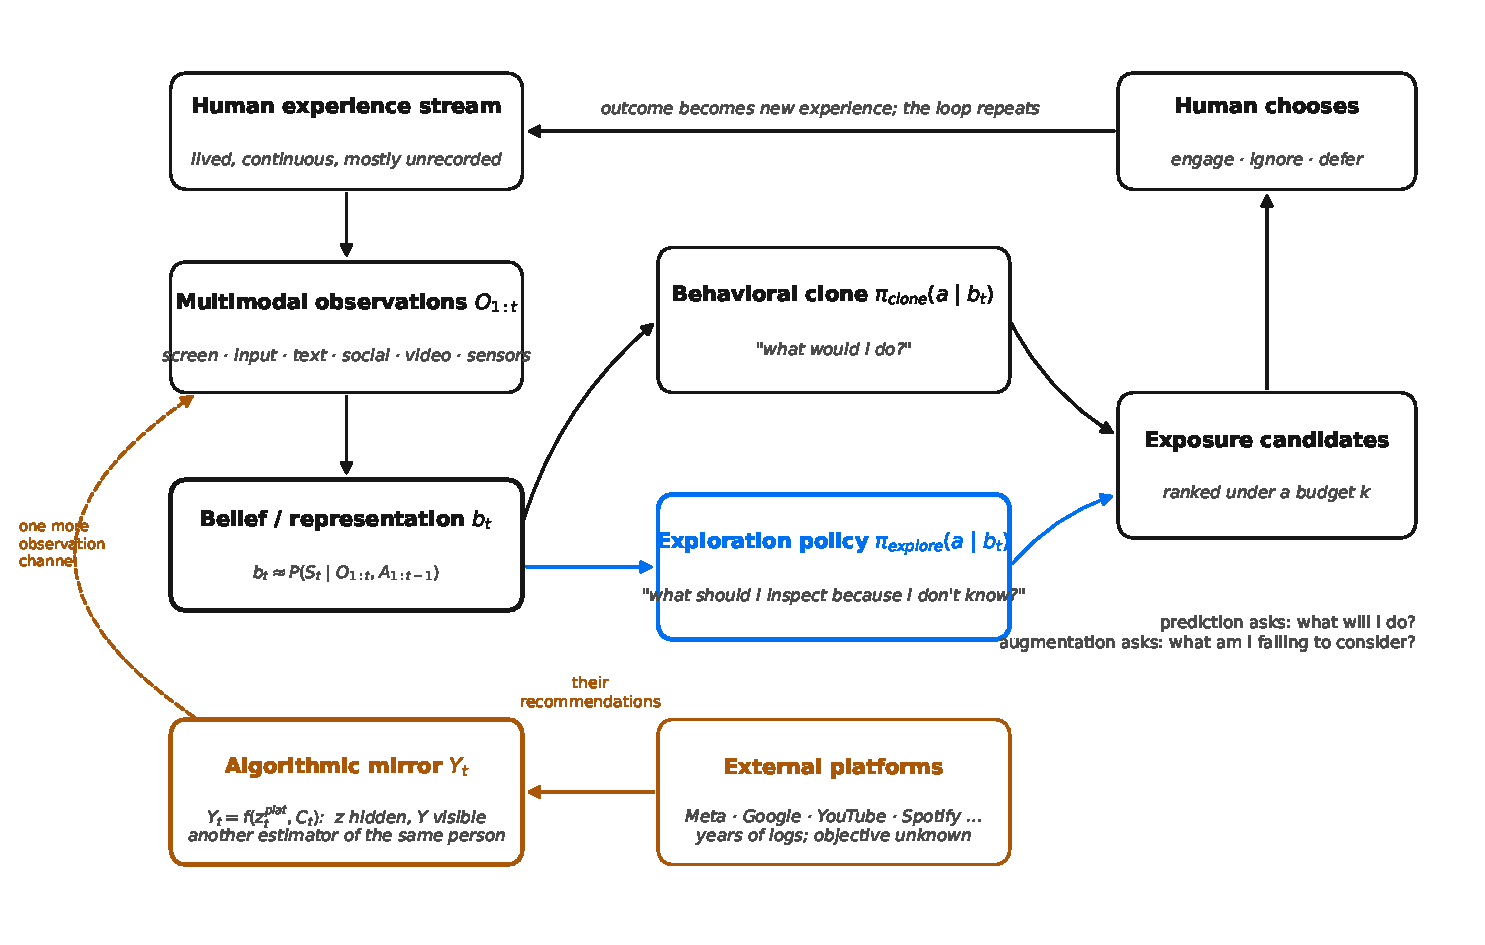
\includegraphics[width=\linewidth]{fig1_architecture.pdf}
\caption{The setting. Observations of a person feed a belief or representation $b_t$. A behavioral clone predicts what the person would do; an exploration policy proposes what to inspect because the model does not know. Both produce exposure candidates, the person chooses, and the outcome becomes new experience. Platforms that have logged the person for years emit recommendations that can be treated as one more observation channel (an ``algorithmic mirror''). This paper tests exploitation and exploration rankers on logged exposures; the mirror channel is proposed, not tested (Section~\ref{sec:mirrors}).}
\label{fig:arch}
\end{figure}

We distinguish four objects (Figure~\ref{fig:arch}). The observed history $O_{1:t}$ is everything logged up to time $t$. A representation $b_t \approx P(S_t \mid O_{1:t}, A_{1:t-1})$ summarizes it; we make no claim that a unique latent ``state of the person'' exists, and $b_t$ can be any learned summary, including a predictive-state representation \citep{littman2002predictive,singh2004predictive}. The behavioral clone $\pi_{\mathrm{clone}}(a \mid b_t)$ predicts the person's action. The augmenting policy $\pi_{\mathrm{aug}}(a \mid b_t)$ decides what to surface. The full problem is a partially observable Markov decision process (POMDP) \citep{kaelbling1998planning}, and with uncertainty about the person's own preferences it becomes a Bayes-adaptive one \citep{duff2002optimal,guez2012efficient}. The data do not support that problem. They contain exposures and the person's responses under his own, unknown policy, with no interventions. We therefore study a narrower retrospective ranking problem with contextual-bandit-style scoring terms \citep{li2010contextual}, evaluated offline \citep{li2011unbiased,swaminathan2015counterfactual}.

\paragraph{Exposures and outcomes.} Messages in a thread form \emph{bursts}: a burst starts with any message that follows at least 24 hours of silence in that thread. An \emph{exposure} (equivalently, a contact event) is a burst that starts with an inbound message. A \emph{weak-tie exposure} is either the first message in a thread or one that arrives after at least 180 days of silence; this is an operational definition, not a measure of tie strength in the sociological sense \citep{granovetter1973strength}. Threads are platform-specific and include group threads. The observed action is whether the subject replied within seven days. The delayed outcome, called Tier A in our protocol and computed automatically, is that within 365 days after the exposure the thread contained at least five further bursts in either direction and at least one message in the last 90 days of that year. We call such exposures \emph{later-lasting}. The outcome is used only as a label, never as a feature.

\paragraph{Scores.} A pure exploitation ranker orders candidates by predicted engagement $\hat{p}(\text{reply} \mid x, b_t)$. The exploration scores we test are
\begin{equation}
s(x) = w_r\,\mathrm{rel}(x) + w_u\,\mathrm{unc}(x) + w_n\,\mathrm{nov}(x) + w_i\,\mathrm{IG}(x) + w_o\,\mathrm{OV}(x) - w_c\,\mathrm{cost}(x).
\label{eq:hybrid}
\end{equation}
Here $\mathrm{rel}$ is the ensemble mean of $\hat{p}$ and $\mathrm{unc}$ its standard deviation across ensemble members. $\mathrm{IG}$ is the disagreement term of Bayesian active learning by disagreement (BALD) \citep{houlsby2011bayesian}: the mutual information between the reply and the ensemble member. It measures what the engagement model would learn about its own parameters, and we use it only as a crude stand-in for the information gain $H(b_t) - \mathbb{E}[H(b_{t+1}) \mid x]$ about the person. $\mathrm{nov}$ is 1 for the first message in a thread and $1/(1+n)$ for a thread with $n$ earlier contact events. $\mathrm{OV}$ is a language-model judgment of how much engaging would open new people, communities or projects, and $\mathrm{cost}$ grows with message length. Each term is a proxy, and whether any of them helps is the question.

\section{Related work}

\paragraph{Belief-state control and Bayes-adaptive exploration.} POMDPs formalize acting under partial observability \citep{kaelbling1998planning}; Bayes-adaptive Markov decision processes (MDPs) make uncertainty about the environment part of the state, so that exploring is optimal when it pays for itself \citep{duff2002optimal,guez2012efficient}. Predictive-state representations replace latent state with predictions of future observations \citep{littman2002predictive,singh2004predictive}, which suits a setting in which no one can name the true state of a person. Continuing, experience-driven learning is the frame of \citet{sutton2018reinforcement} and \citet{silver2025era}.

\paragraph{Exploration and intrinsic motivation.} Optimism under uncertainty, as in upper-confidence-bound (UCB) methods \citep{auer2002finite}, posterior sampling \citep{thompson1933likelihood,russo2018tutorial}, information gain \citep{houlsby2011bayesian}, curiosity \citep{schmidhuber2010formal,pathak2017curiosity} and empowerment \citep{klyubin2005empowerment} each justify taking actions of uncertain immediate value. Our hybrid score borrows one proxy from several of these traditions.

\paragraph{Recommendation, serendipity and feedback loops.} Contextual bandits are the standard framing for exploration in recommendation \citep{li2010contextual}, and off-policy estimators make logged data usable for evaluation \citep{li2011unbiased,swaminathan2015counterfactual}. Serendipity and diversity have long been proposed as correctives to accuracy-only ranking \citep{ziegler2005improving,kotkov2016survey}, and recommender feedback loops are known to homogenize what users see \citep{chaney2018algorithmic}. We evaluate these ideas for a single person over a long horizon rather than across many users over short ones.

\paragraph{Weak ties.} That novel information and opportunity tend to arrive through weak ties is an old sociological claim \citep{granovetter1973strength}, recently supported by a large field experiment on a professional network \citep{rajkumar2022causal}. Our outcome is narrower: whether a weak-tie exposure grew into a lasting thread, not what it led to.

\paragraph{Imitation and lifelogging.} Behavioral cloning and its compounding-error problem are classical \citep{pomerleau1991efficient,ross2011reduction}. Lifelogging research documents the capture and retrieval of personal data \citep{gurrin2014lifelogging}; we use such an archive to test decision policies rather than for retrieval.

\section{Data}
\label{sec:data}

\paragraph{Subject and archive.} The subject is the author. He began keeping digital records in secondary school and later added continuous screen, input, audio, location and wearable capture. Messages (Table~\ref{tab:sources}) are the only modality we have processed across the full fifteen years. A second long-running record exists but is not used here: 916 videos the subject streamed or uploaded to YouTube between 2016 and 2026, about 700 hours in total, almost all of it since 2021 and much of it live sessions of him working or playing. Denser capture streams (screen, input, attention, location, cameras) exist only from July to September 2026 and are used here only by the behavioral-cloning experiment. Platform exports fall into two kinds. Activity logs of the subject's own actions, such as watch and search history, span years. Records of what recommenders showed him (a feed-exposure log, suggested people, inferred ad interests) exist only as single snapshots from July to September 2026 (Section~\ref{sec:mirrors}).

\begin{table}[t]
\centering
\small
\begin{tabular}{lrrr}\toprule
Source & First year & Messages & Contact events\\\midrule
Facebook Messenger & 2011 & 2,610,864 & 20,156\\
Telegram & 2016 & 363,225 & 5,759\\
Instagram DMs & 2017 & 72,345 & 4,491\\
Discord & 2020 & 21,622 & 2,467\\
Gmail (3 accounts) & 2013 & 6,482 & 1,114\\
LinkedIn & 2020 & 3,104 & 489\\
Twitter DMs & 2016 & 2,223 & 216\\
Google Voice & 2024 & 2,072 & 405\\
Google Chat & 2016 & 656 & 71\\
\midrule
Total & & 3,082,593 & 35,168\\\bottomrule
\end{tabular}

\caption{Message sources, 2011-11 to 2026-09-15. Messages are normalized into one event schema with hashed thread identifiers. A contact event is a burst that starts with an inbound message.}
\label{tab:sources}
\end{table}

\paragraph{Exposure table.} From 3{,}082{,}593 messages in 7{,}139 threads we extract 35{,}168 contact events. Of these, 2{,}856 open a new thread and 863 revive a thread silent for at least 180 days, giving 3{,}719 weak-tie exposures. Of the 3{,}221 weak-tie exposures whose 365-day outcome window is complete, 430 (13.3\%) became later-lasting. The corresponding rate over all contact events is much higher (63\%), because most contact events come from existing strong ties. We therefore rank weak-tie exposures only.

\paragraph{Candidate pools and split.} Rankings are made per ISO week among that week's weak-tie exposures. The primary pool excludes messages that a local judge rates as automated, bulk or marketing (probability above 0.5, \gemmaAutoPct\% of weak-tie exposures); the secondary pool keeps them. The split is chronological: train through 2019-12-31, validation 2021-01-01 to 2022-12-31, test from 2024-01-01. The years 2020 and 2023 are embargoes that belong to no split; each is at least as long as the 365-day outcome horizon, so no training or validation label depends on events in a later split. Test exposures can run up to 2025-09-15, the last date with a complete outcome window. Table~\ref{tab:pools} gives the counts. The share of weak-tie exposures that became later-lasting falls over time (primary pool: \nPTrRate\% in train, \nPVaRate\% in validation, \nPTeRate\% in test), so absolute metrics are not comparable across splits. Paired comparisons within a split are unaffected, though their size still depends on that split's candidate-set sizes.

\begin{table}[t]
\centering
\small
\begin{tabular}{lrrrr}\toprule
 & \multicolumn{2}{c}{Primary pool} & \multicolumn{2}{c}{Secondary pool}\\
\cmidrule(lr){2-3}\cmidrule(lr){4-5}
Split & Exposures & Became lasting & Exposures & Became lasting\\\midrule
Train (2011--2019) & 466 & 106 & 776 & 140\\
Validation (2021--2022) & 672 & 113 & 905 & 134\\
Test (2024--2025) & 393 & 36 & 738 & 52\\
\bottomrule
\end{tabular}

\caption{Weak-tie exposures with complete 365-day outcomes, per split and pool. Train and validation were used for development; test was opened once after pre-registration (see the disclosure in Section~\ref{sec:methods}).}
\label{tab:pools}
\end{table}

\paragraph{Privacy.} Bulk processing of message text (embeddings and judgments) ran on local models on the subject's own machines: two Apple Silicon computers and a desktop with two consumer GPUs. No bulk message text, contact identity or raw export was sent to an external service. The paper and the code repository contain only aggregate statistics and hashed exposure identifiers.

\section{Methods}
\label{sec:methods}

\paragraph{Leakage control.} Every feature for an exposure at time $t$ is computed from events timestamped at or before $t$. Outcome columns are declared in the schema as label-only, and the feature builder refuses any frame that contains one. Tests inject each label column into feature frames and check that they are rejected, and check that the split is monotone and embargoed.

\paragraph{Features.} Three tiers. (i) Metadata: whether the thread is new or dormant, group size, prior message counts in each direction, prior reply rate in the thread, recency, thread age, the subject's global activity over the previous 30 days, the platform's share of all the subject's earlier contact events, message length, hour and weekday. (ii) Content: a local multilingual sentence encoder (\texttt{paraphrase-multilingual-MiniLM-L12-v2} \citep{reimers2019sentence,reimers2020making}) embeds each inbound message and 396{,}381 of the subject's own messages; we use 32 principal components fit on training data and the maximum and mean cosine similarity to the subject's own messages in the preceding 90 days. (iii) Typed judgments: six questions per message (invites to an event or opportunity; expects a reply; written on behalf of an organization; automated or marketing; an option-value score on four described levels; a six-way message type), answered by a local model and read from its next-token distribution restricted to the answer labels. We use the open-source AnyJev library (version 0.0.1) \citep{anyjev2026} at its zero-label level L0, which averages option-order bias over rotations of the answer labels and divides out the label prior. The primary judge is Gemma 4 31B \citep{gemmateam2026gemma4}, quantized with activation-aware weight quantization (AWQ) and served locally with vLLM \citep{kwon2023efficient}.\footnote{Checkpoint \texttt{QuantTrio/gemma-4-31B-it-AWQ} on Hugging Face.} Qwen3-8B \citep{yang2025qwen3}, 8-bit on Apple Silicon, is a second, independent judge for the weak-tie exposures.

\paragraph{Engagement model.} A five-member bootstrap ensemble of logistic regressions predicts reply-within-seven-days from all three feature tiers. It is fit on the 8{,}052 contact events of the training period, strong and weak ties alike, and on nothing later. Its mean is $\mathrm{rel}(x)$ and its spread is $\mathrm{unc}(x)$.

\paragraph{Policies.} Relevance-only, the ensemble mean, is our stand-in for a recommender driven by a model of the subject's own engagement. UCB adds the ensemble spread to relevance with coefficient 1. Thompson sampling draws from a Gaussian with the ensemble mean and spread. $\varepsilon$-greedy uses $\varepsilon = 0.2$. The hybrid score is Eq.~\ref{eq:hybrid} with $w_r = 1$, $w_c = 0.25$ and the other four weights chosen from $\{0, 0.25, 0.5, 1\}$ by grid search on the preceding split, maximizing recall at 5. New-thread-first ranks by $\mathrm{nov}$.\footnote{The pre-registration calls this policy ``new-person-first''. We renamed it after the freeze because a new thread only approximates a new person.} Platform popularity ranks by the platform's share of earlier contact events. Random is a uniform shuffle. Random with a diversity budget is a control: it fills the top of the list with one exposure per platform, in random order, before ranking the rest randomly. Stochastic policies, and policies with many ties, are averaged over 20 seeds per week.

\paragraph{Metrics and statistics.} A week is scored if it contains at least one later-lasting exposure. Within a scored week, reciprocal rank is averaged over its later-lasting exposures, and recall at $k$ is the share of them ranked in the top $k$. Mean reciprocal rank (MRR) and recall are then averaged over scored weeks. Comparisons are paired by week and summarized by the mean difference with a 95\% cluster-bootstrap interval over weeks (5{,}000 resamples); intervals for single-policy MRR use 2{,}000 resamples. Reply prediction is summarized by the area under the ROC curve (AUC).

\paragraph{Pre-registration.} We froze the annotation protocol and the analysis plan in a git commit and tag (\texttt{annotation-v1}) and pushed it to the public repository. GitHub recorded the push at 19:16:34 UTC on 2026-09-27; the test split was opened eight seconds later with the recorded commands. Before submission we rewrote the repository history to remove personal account names from two files; commit identifiers changed but contents and timestamps did not, and the repository lists the mapping from original to rewritten commits. Three hypotheses carry decision rules, each on the paired MRR difference in the primary pool (Table~\ref{tab:prereg}). \textbf{H-PREM}: relevance-only ranks later-lasting weak ties below random; supported if the interval lies below zero, rejected if above. \textbf{H-SER}: the hybrid exploration score beats random exploration with an equal diversity budget; supported only if the interval lies above zero, rejected otherwise. \textbf{H-NOV}: new-thread-first beats the same baseline; supported if the interval lies above zero, rejected if below, inconclusive otherwise. Paired recall differences are pre-registered secondary endpoints without decision rules (Appendix Table~\ref{tab:secondary}).

\paragraph{Disclosure: a pre-freeze look at pooled outcome aggregates.} Before the freeze, we computed descriptive statistics that pooled every period, including the test years. They were the outcome base rates for all contact events and for weak-tie exposures, and the associations between the judgments and the outcome. Our development report also printed the size of the test pool (738 weak-tie exposures, 52 later-lasting). These pooled aggregates informed three choices: ranking weak-tie exposures only, filtering automated messages from the primary pool, and our reading of the option-value term. No policy was ranked on test data before the freeze. The per-period breakdown in Table~\ref{tab:judgments} and Appendix Table~\ref{tab:judgments_test} was computed after it. The secondary pool applies no automated filter, and applying the same decision rules to it gives the same three outcomes.

\section{Results}
\label{sec:results}

\subsection{The subject's next action is partly predictable}

An earlier experiment on the same subject, pre-specified in an internal protocol, asked a frozen Qwen3-8B to pick the subject's actual next action among five candidates drawn from his own history (chance 20\%). Candidates are scored by pointwise mutual information between each candidate and the situation, and ties count against the correct answer. Test cases come from 2026-08-25 to 2026-09-14; the adapter's training data end on 2026-08-17. Seven action families were covered (reply, send, type, speak, copy, click, look). The pooled results exclude the speak family ($n = 312$), as its protocol specified. The protocol was amended during the experiment; an interim pass and two baseline variants had been scored on test cases before some amendments, and the final amendment for the scores reported here was committed before they were computed. We recomputed the results from the raw per-case scores (Table~\ref{tab:clone}).

Given only the immediate situation, the base model reaches 28.0\% top-1. A LoRA adapter \citep{hu2022lora} trained on the subject's own text for 600 steps, the pre-registered checkpoint, reaches 37.8\%, a gain of 9.8 points with an interval of $[6.8, 13.4]$ from a bootstrap over 302 session or app-hour clusters, and improves on 20 of 21 test days. Of the protocol's four hypotheses, only this one held. Adding every available context layer to the base model did not help (H1, $-2.4$ points $[-4.6, 0.2]$); relevant personal history did not beat an equal amount of random history (H2, $-0.3$ $[-2.0, 1.2]$); and a separate event-sequence model did not gain from all layers over the target family's own layer (H4, $+0.4$ $[-2.2, 2.9]$). Shuffled or random-history controls sit at 24 to 25\%. Two caveats. Among the pooled families, seventeen of the 21 test days contain only reply and send decisions. The adapter also loses on the copy, click and look families. It captures the subject's writing better than his screen behavior.

\begin{table}[t]
\centering
\small
\begin{tabular}{lrrrr}\toprule
Variant & Top-1 & $\Delta$ vs.\ A (pts) & 95\% CI & Days with gain\\\midrule
A: immediate situation & 0.280 & & & \\
C: relevant personal history & 0.245 & $-$3.5 & [$-$5.7, $-$1.6] & 6/21\\
F: random history & 0.248 & $-$3.2 & [$-$5.4, $-$1.2] & 5/21\\
E: all context layers, base model & 0.256 & $-$2.4 & [$-$4.6, 0.2] & 7/21\\
E-shuf: shuffled context & 0.241 & $-$4.0 & [$-$6.1, $-$1.4] & 4/21\\
L: A + personal LoRA & 0.378 & 9.8 & [6.8, 13.4] & 20/21\\
L+E: all layers + personal LoRA & 0.382 & 10.1 & [7.0, 14.1] & 19/21\\
\bottomrule
\end{tabular}

\caption{Five-way next-action prediction, pooled over six action families ($n = 1{,}695$), recomputed from raw per-case scores. Intervals are bootstraps over 302 session or app-hour clusters. Of four pre-specified hypotheses, only the personal adapter (L $>$ A) held.}
\label{tab:clone}
\end{table}

\subsection{A relevance ranker buries later-lasting ties, and the hybrid exploration score does not recover them}

Table~\ref{tab:prereg} gives the three pre-registered decisions and Table~\ref{tab:policies} the policy-level results. The engagement model is informative about replies: AUC \aucPrimaryTest{} on the \nPTeExp{} primary-pool test exposures (\aucSecondaryTest{} on the secondary pool). As a ranker for later-lasting ties, however, it does worse than random order on the held-out years: MRR 0.327 against 0.465, a paired difference of $-0.138$ $[-0.200, -0.067]$. H-PREM is supported, and the direction matches validation.

The hybrid score, with weights tuned on validation (relevance 1, novelty 0.5, option value 1, cost 0.25; uncertainty and information gain received weight 0), scored MRR 0.279. It fell below random exploration with a diversity budget (0.496) by $-0.217$ $[-0.267, -0.164]$. H-SER is rejected. UCB and Thompson sampling, which add epistemic uncertainty to the relevance model, track relevance-only closely (0.305 and 0.328). With the relevance signal as their base, they inherit its ranking.

New-thread-first was the best non-random policy on validation (MRR 0.440 against 0.418 for random with diversity). It did not replicate on test: the difference is $-0.035$ $[-0.085, 0.013]$, an interval that includes zero around a negative point estimate. H-NOV is inconclusive. The secondary pool, which keeps automated messages, gives the same three verdicts: relevance minus random $-0.126$ $[-0.174, -0.065]$, hybrid minus random with diversity $-0.157$ $[-0.193, -0.116]$, new-thread-first minus random with diversity $-0.027$ $[-0.067, 0.014]$ (Appendix Table~\ref{tab:policies2}). The pre-registered recall endpoints agree in sign (Appendix Table~\ref{tab:secondary}). Figure~\ref{fig:forest} shows validation and test side by side, and Figure~\ref{fig:timeline} shows every later-lasting test exposure.

\begin{table}[t]
\centering
\footnotesize
\resizebox{\linewidth}{!}{\begin{tabular}{lllllll}\toprule
Hypothesis & MRR difference & Supported if & Validation & Test & Test, labels permuted & Test verdict\\\midrule
H-PREM & relevance $-$ random & CI $<0$ & $-$0.061 [$-$0.113, $-$0.002] & $-$0.138 [$-$0.200, $-$0.067] & 0.020 [$-$0.067, 0.110] & \textbf{supported}\\
H-SER & hybrid $-$ random w/ diversity & CI $>0$ & $-$0.044 [$-$0.107, 0.028] & $-$0.217 [$-$0.267, $-$0.164] & $-$0.013 [$-$0.114, 0.092] & \textbf{rejected}\\
H-NOV & novelty $-$ random w/ diversity & CI $>0$ & 0.021 [$-$0.018, 0.060] & $-$0.035 [$-$0.085, 0.013] & 0.007 [$-$0.058, 0.072] & \textbf{inconclusive}\\
\bottomrule
\end{tabular}}

\caption{Pre-registered hypotheses, primary pool: paired per-week MRR differences with 95\% cluster-bootstrap intervals over scored weeks (validation \nPVaScored{} weeks, test \nPTeScored{} weeks). H-PREM is relevance-only minus random. H-SER is the hybrid score minus random with a diversity budget. H-NOV is new-thread-first minus the same baseline. Decision rules are in Section~\ref{sec:methods}. The permuted column shuffles outcome labels within each test week; every interval then includes zero, as it should.}
\label{tab:prereg}
\end{table}

\begin{table}[t]
\centering
\small
\begin{tabular}{lrrrr}\toprule
 & \multicolumn{2}{c}{Validation 2021--2022} & \multicolumn{2}{c}{Held-out test 2024--2025}\\
\cmidrule(lr){2-3}\cmidrule(lr){4-5}
Policy & MRR & recall@1 & MRR [95\% CI] & recall@1\\\midrule
Relevance-only (reply model) & 0.347 & 0.152 & 0.327 [0.24, 0.42] & 0.100\\
UCB (relevance + uncertainty) & 0.333 & 0.134 & 0.305 [0.23, 0.38] & 0.067\\
Thompson sampling & 0.352 & 0.152 & 0.328 [0.24, 0.42] & 0.115\\
Hybrid exploration score & 0.374 & 0.167 & 0.279 [0.23, 0.33] & 0.017\\
$\varepsilon$-greedy ($\varepsilon=0.2$) & 0.389 & 0.189 & 0.399 [0.33, 0.47] & 0.193\\
Random & 0.408 & 0.187 & 0.465 [0.41, 0.52] & 0.215\\
Random with diversity budget & 0.418 & 0.190 & 0.496 [0.44, 0.56] & 0.257\\
New-thread-first (novelty) & 0.440 & 0.219 & 0.462 [0.39, 0.53] & 0.223\\
Platform popularity$^\dagger$ & 0.413 & 0.209 & 0.552 [0.43, 0.67] & 0.350\\
\bottomrule
\end{tabular}

\caption{Ranking later-lasting weak-tie exposures, primary pool. Test: \nPTeExp{} exposures over \nPTeWeeks{} weeks; the \nPTeScored{} scored weeks contain \nPTeScoredExp{} exposures, \nPTePos{} of them later-lasting (median \nPTeMedian{} per scored week). Validation: \nPVaExp{} exposures; \nPVaScored{} scored weeks with \nPVaScoredExp{} exposures, \nPVaPos{} later-lasting (median \nPVaMedian{}). $^\dagger$The policy was run as registered, but its comparison with the baselines was not pre-registered; see Section~\ref{sec:exploratory}.}
\label{tab:policies}
\end{table}

\begin{figure}[t]
\centering
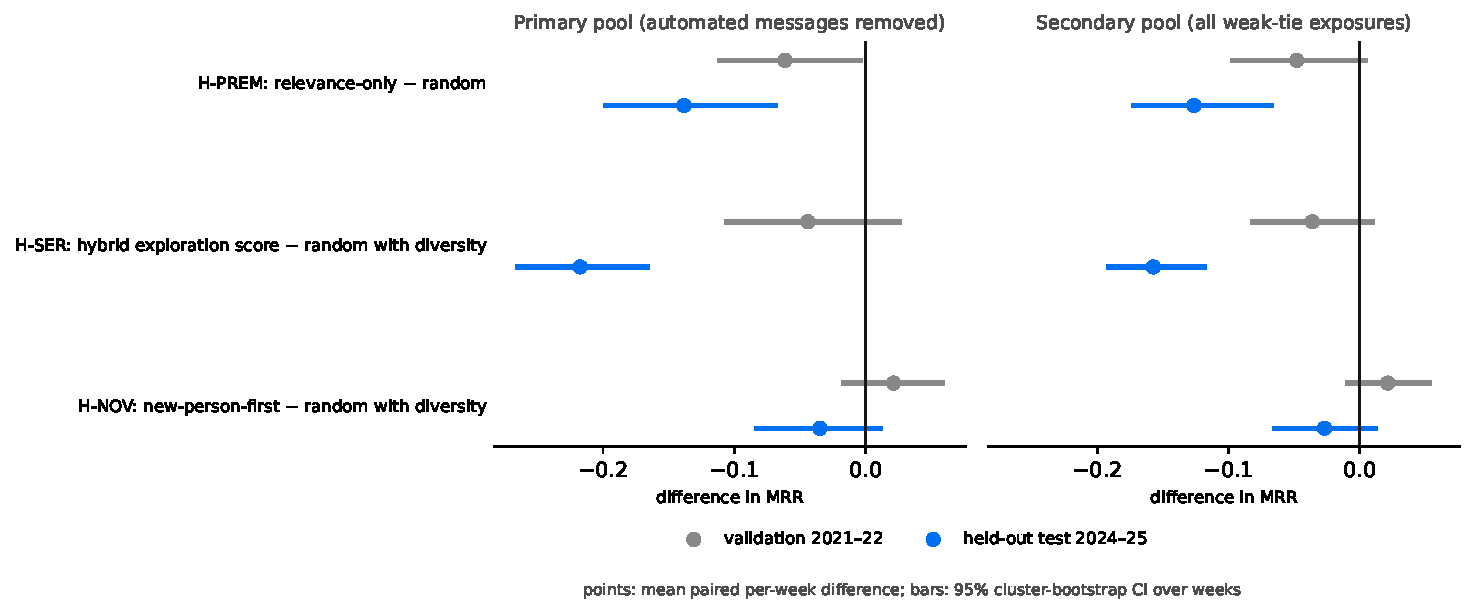
\includegraphics[width=\linewidth]{fig4_preregistered.pdf}
\caption{Pre-registered comparisons on validation (gray) and on the held-out test years (blue), for both candidate pools. Negative values mean the first policy ranks later-lasting ties worse.}
\label{fig:forest}
\end{figure}

\begin{figure}[t]
\centering
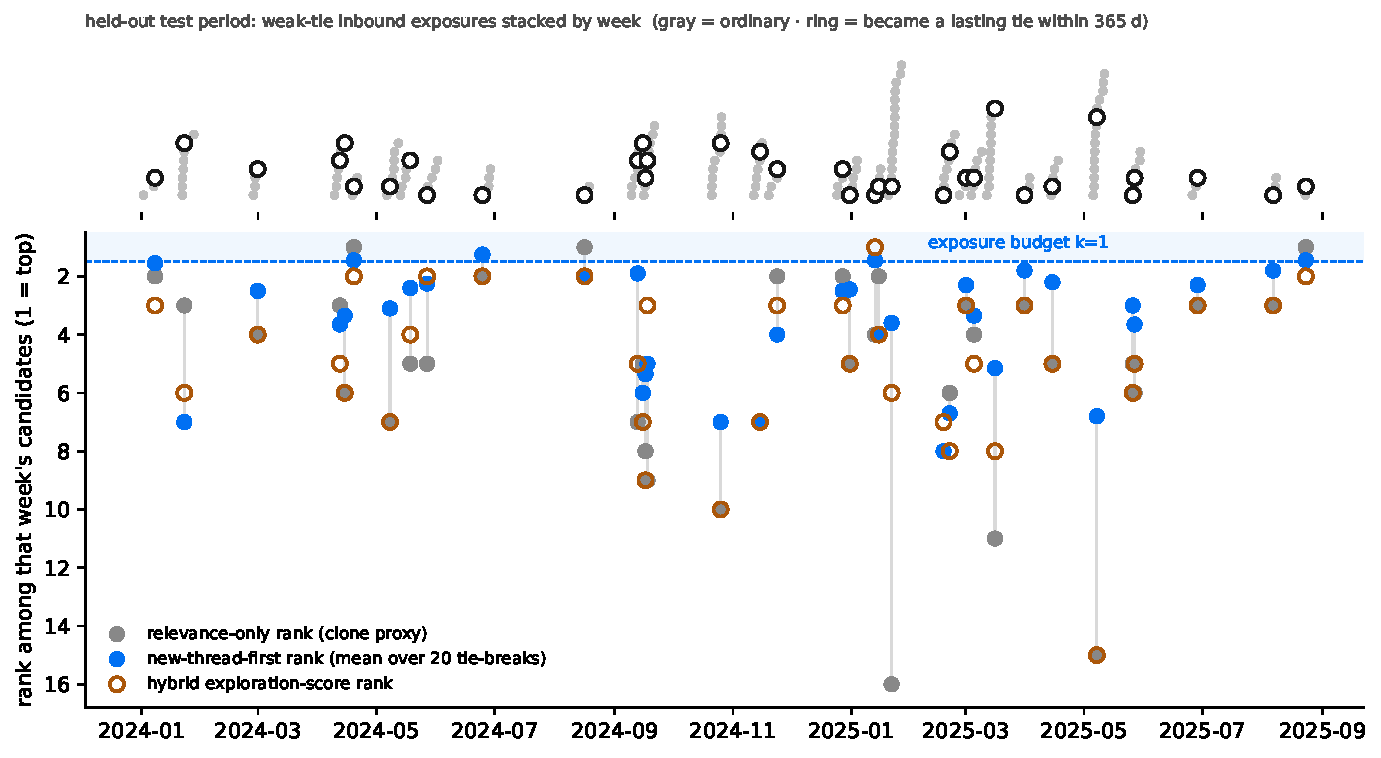
\includegraphics[width=\linewidth]{fig2_counterfactual.pdf}
\caption{Held-out test period, primary pool, scored weeks. Top: weak-tie inbound exposures stacked by week; rings mark those that became lasting ties. Bottom: the weekly rank of each later-lasting exposure under relevance-only (gray), new-thread-first (blue, averaged over tie-breaks) and the hybrid score (hollow). The shaded band is a budget of one exposure per week. No identities or message content are shown.}
\label{fig:timeline}
\end{figure}

\subsection{What the later-lasting exposures looked like}

Table~\ref{tab:judgments} compares typed judgments of later-lasting and ordinary weak-tie exposures in the development years (before 2024), and Appendix Table~\ref{tab:judgments_test} does the same for the test years. The two judges agree on direction. Later-lasting exposures were less often invitations to an event, job, project or community, less often written on behalf of an organization, and more often personal or social chat. The judged option value, the term meant to capture ``this could open doors'', carried no signal in the development years (AUC 0.51 and 0.46) and was weakly inverse in the test years (0.42 and 0.39).

Agreement between the judges on the binarized judgments is substantial for invitation (Cohen's $\kappa = 0.70$), organization (0.67) and marketing (0.67), moderate for the message type ``social'' (0.60), and only fair for ``automated'' (0.37) and ``expects a reply'' (0.38). The judges disagree most about what counts as automated: Gemma flags \gemmaAutoPct\% of weak-tie exposures, Qwen \qwenAutoPct\%. On validation, re-running the primary analysis with Qwen's filter (and, in that run, an engagement model fit on weak-tie exposures only) left the ordering relevance $<$ hybrid $<$ random $<$ random with diversity $<$ new-thread-first unchanged; the position of UCB moved.

These patterns suggest one reason the hybrid score did not help. It inherits most of its ordering from the relevance term (hybrid minus relevance on test: $-0.048$ $[-0.118, 0.014]$), and its largest added weight went to option value, which in this record did not identify the exposures that lasted. We did not test this explanation directly.

\begin{table}[t]
\centering
\small
\resizebox{\linewidth}{!}{\begin{tabular}{lrrrrrr}\toprule
 & \multicolumn{3}{c}{Gemma 4 31B} & \multicolumn{3}{c}{Qwen3-8B}\\
\cmidrule(lr){2-4}\cmidrule(lr){5-7}
Judgment & Ordinary & Became lasting & AUC & Ordinary & Became lasting & AUC\\\midrule
Invites to an event, job, project or community & 0.21 & 0.11 & 0.49 & 0.12 & 0.04 & 0.48\\
Written on behalf of an organization or group & 0.28 & 0.12 & 0.43 & 0.17 & 0.03 & 0.42\\
Automated, bulk or marketing & 0.34 & 0.19 & 0.38 & 0.08 & 0.02 & 0.47\\
Option-value score (0--3) & 1.07 & 1.07 & 0.51 & 1.73 & 1.62 & 0.46\\
Type: personal or social chat & 0.41 & 0.58 & 0.61 & 0.48 & 0.57 & 0.57\\
\bottomrule
\end{tabular}}

\caption{Development years (before 2024; \nDevJudged{} weak-tie exposures, \nDevJudgedPos{} later-lasting): mean judged probability, or score for option value, for ordinary and later-lasting exposures with complete outcomes, and each judgment's AUC for the outcome. Both judges ran locally at AnyJev level L0 with zero labels.}
\label{tab:judgments}
\end{table}

\subsection{Controls}

\paragraph{Label permutation.} Shuffling outcome labels within each test week removes every effect: all three pre-registered intervals include zero (Table~\ref{tab:prereg}). Across the 24 permuted comparisons we computed (six policy pairs, four metrics), one interval touches zero at its edge, consistent with chance.

\paragraph{Leakage.} The leakage and split tests passed at the tagged commit and on every run.

\subsection{Exploratory observations}
\label{sec:exploratory}

These analyses were not pre-registered and should be read as hypotheses.

\paragraph{Platform.} Ranking by the platform's share of the subject's earlier contact events had the highest test MRR of any policy (0.552). Its paired difference from random with diversity was $+0.056$ $[-0.040, 0.155]$ on the primary pool and $+0.091$ $[-0.001, 0.186]$ on the secondary pool; both intervals include zero. The share is cumulative since 2011, so it reflects the platforms that dominated the subject's history more than where he was active at the time. If the effect is real, the platform a message arrives on predicts whether its thread lasts. It is also confounded: the subject moved between platforms over the years, and a platform's share encodes both habit and era.

\paragraph{Feature tiers.} After the freeze we compared engagement models built from subsets of the features. Reply-prediction AUC on the primary pool (validation/test) was 0.606/0.618 with metadata alone, 0.644/0.626 with content embeddings, 0.670/0.668 with typed judgments, and 0.666/0.671 with all three. We did not compute ranking metrics per tier.

\paragraph{Exploration over fifteen years.} Figure~\ref{fig:proxies} shows monthly proxies computed from message metadata only. The subject's reply rate to first messages from new threads has stayed near 0.5 since 2017. Self-initiated new threads grew rather than shrank, from about 100 in 2016 to between roughly 290 and 580 a year from 2017 to 2025. The motivating intuition was that the subject explored more as a teenager than as an adult. These data cannot test it: counts before 2016 are too small to read, and the proxies are confounded by platform coverage (bottom panel).

\begin{figure}[t]
\centering
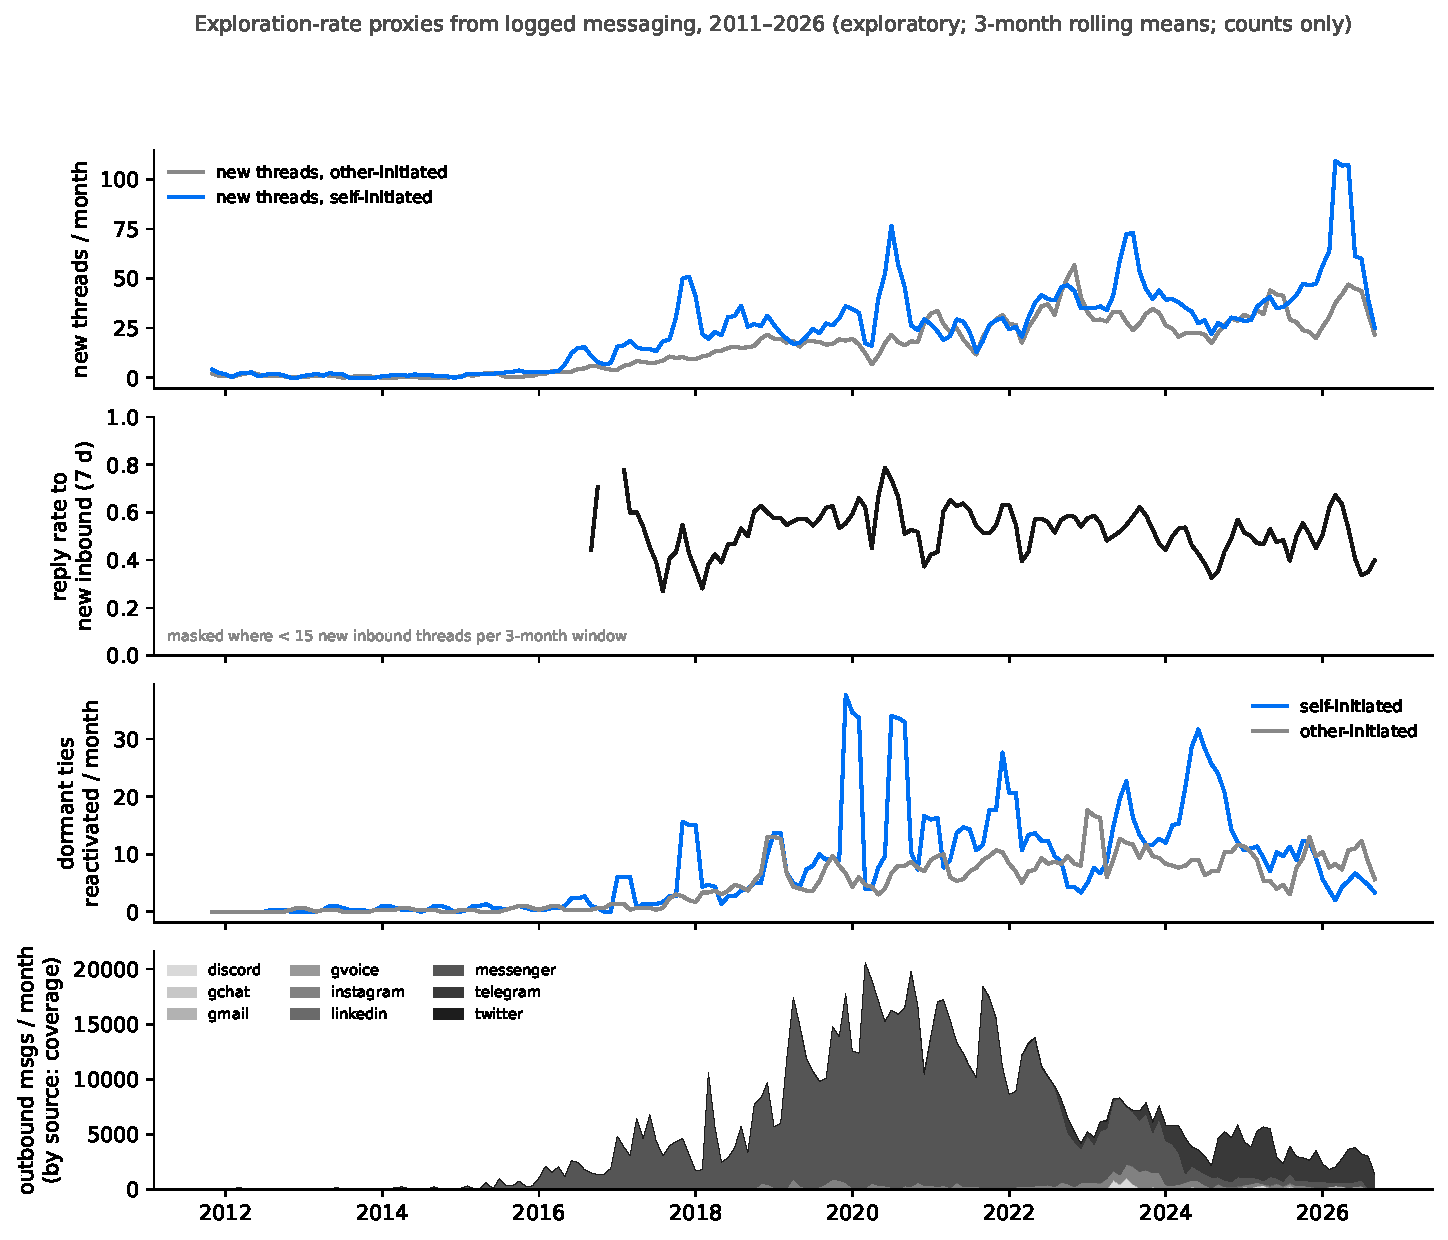
\includegraphics[width=0.78\linewidth]{fig3_exploration_proxies.pdf}
\caption{Exploratory exploration-rate proxies from message metadata, 2011 to 2026 (three-month rolling means). Reply rate is masked where fewer than 15 new inbound threads fall in a window. The bottom panel shows outbound volume by platform, to make platform migration visible.}
\label{fig:proxies}
\end{figure}

\section{Algorithmic mirrors: proposed, not tested}
\label{sec:mirrors}

Large platforms maintain learned representations of each user and expose only their outputs. A feed, a list of suggested people or a set of inferred ad interests is a noisy observation of the platform's estimate of the user: $Y_t = f(z^{\mathrm{plat}}_t, C_t)$ with $z^{\mathrm{plat}}_t$ hidden. For a personal agent these outputs are an unusual observation channel. They are another model's estimate of the same person, trained on behavior the agent may not see, with an objective the agent does not know. Comparing that estimate with the agent's own, and asking whether disagreement predicts later change, is a natural experiment. We could not run it. The subject's exports of recommender outputs (a Facebook feed-exposure log, suggested friends, inferred ad interests, Twitter personalization) are single snapshots taken from July to September 2026, and recommendation surfaces such as home feeds are not exported at all. His long-running activity logs (watch and search history) record his own actions, not what was recommended to him. Testing the mirror idea requires prospective collection of platform outputs over time.

\section{Limitations and ethics}

\paragraph{One subject, who is also the researcher.} Every number here describes one person's record. The contribution is a method, a benchmark design and one pre-registered case, not a population estimate. The dual role invites motivated analysis. The safeguards are the automatic outcome definition, the pre-registration and the single opening of the test split. They are imperfect: pooled outcome aggregates were seen before the freeze (Section~\ref{sec:methods}), and H-SER was already failing on validation, so its rejection on test was expected rather than a surprise.

\paragraph{The outcome is narrow.} ``Later-lasting'' means a thread stayed active and grew. It does not capture a single message that led to a job, a collaborator or an idea without further conversation. It misses ties that moved to another platform, because threads are platform-specific, and it counts group threads, which can grow without any one relationship doing so. For the same reason, ``new thread'' is only an approximation of ``new person''. Manual labels of a blind 300-exposure sample, collected after the freeze and analysed separately, will test whether the conclusions hold for outcomes the subject judges consequential.

\paragraph{Observational and retrospective.} We rank exposures that occurred. We cannot say what would have happened if an agent had surfaced different ones, and nothing here licenses causal claims about any exposure. Platforms also chose which messages reached the subject at all.

\paragraph{Small test set.} The primary test pool has \nPTeScored{} scored weeks with a median of \nPTeMedian{} candidates each. Intervals are correspondingly wide.

\paragraph{Third parties.} Other people's messages were processed by local models to compute features and judgments. The cloud-hosted coding assistant also saw a few short excerpts of individual messages during debugging (see the AI-assistance statement). No identity or message content is reported; Figure~\ref{fig:timeline} shows only the week of each later-lasting test exposure. The correspondents did not consent to the analysis, and we limit its outputs to aggregates for that reason.

\section{Discussion}

Three results bear on how personal agents should be built. First, in this record the signal that best predicts what the subject will answer is a poor guide to which new threads will last. The relevance ranker did worse than uninformative on later-lasting ties: it ranked them below random. That is the worry behind engineered serendipity, and here it shows up on held-out years instead of in an anecdote.

Second, the obvious fix did not work. UCB and Thompson sampling inherit the relevance model's ordering, and the tuned hybrid score, built mostly from relevance and a judged option value, fell well below random exploration with a diversity budget. That control needs no model of the person at all, and on MRR no policy we tested beat it with an interval clear of zero. Anyone building a personal agent should measure exploration terms against random-with-coverage before trusting them. A term that encodes the designer's theory of what a good opportunity looks like deserves particular suspicion; ours did not help.

Third, predicting a person and augmenting them are different problems. A small adapter adds ten points to next-action prediction for the same subject, so his short-term behavior is partly predictable. A separate model of his engagement, trained on his earlier years, ranks the exposures that later lasted below random. The two models differ in data and target, so this is consistent with, not proof of, the idea that a clone inherits its source's blind spots.

The stream archive described in Section~\ref{sec:data} is the obvious next source: years of the subject's own screen and camera activity could give the belief state far more than message metadata does. The eventual problem is belief-state control with the person in the loop. The natural next step is prospective: a small daily exposure budget, randomized between policies, with outcomes measured over months. The retrospective benchmark here sets the baseline such a study should beat.

\section{Conclusion}

On fifteen years of one person's inbound messages, a ranker trained to predict his engagement buried the weak-tie exposures that became lasting ties, and a hand-built exploration score did not recover them. On mean reciprocal rank, random exploration with coverage was not beaten by any score we tested. Prediction asks what a person will do; augmentation asks what they are failing to consider. In this record the two came apart, and the exploration terms we borrowed from the literature did not close the gap.

\paragraph{Code and data availability.} Code, tests, the frozen protocol and pre-registration (git tag \texttt{annotation-v1}) and all aggregate results are available at
\begin{center}\url{https://github.com/CarlKho-Minerva/arxiv-Engineering-Serendpity}\end{center}
The underlying messages and exports are private and are not released.

\paragraph{Use of AI assistance.} A cloud-hosted AI coding assistant (Claude, Anthropic) wrote and ran the analysis code on the author's machine, produced the figures and drafted this manuscript under the author's direction. It saw code, aggregate outputs and, occasionally during debugging, short excerpts of individual messages printed to the terminal; bulk text processing used local models only. The author reviewed the analysis and takes responsibility for the content.

\bibliographystyle{plainnat}
\bibliography{refs}

\appendix
\section{Additional tables}

\begin{table}[h]
\centering
\small
\begin{tabular}{lrrrr}\toprule
 & \multicolumn{2}{c}{Validation 2021--2022} & \multicolumn{2}{c}{Held-out test 2024--2025}\\
\cmidrule(lr){2-3}\cmidrule(lr){4-5}
Policy & MRR & recall@1 & MRR [95\% CI] & recall@1\\\midrule
Relevance-only (reply model) & 0.296 & 0.115 & 0.193 [0.15, 0.25] & 0.038\\
UCB (relevance + uncertainty) & 0.288 & 0.115 & 0.181 [0.14, 0.24] & 0.026\\
Thompson sampling & 0.298 & 0.112 & 0.192 [0.15, 0.25] & 0.039\\
Hybrid exploration score & 0.310 & 0.106 & 0.182 [0.15, 0.23] & 0.013\\
$\varepsilon$-greedy ($\varepsilon=0.2$) & 0.329 & 0.136 & 0.275 [0.24, 0.31] & 0.106\\
Random & 0.343 & 0.135 & 0.320 [0.29, 0.35] & 0.107\\
Random with diversity budget & 0.346 & 0.117 & 0.339 [0.31, 0.38] & 0.124\\
New-thread-first (novelty) & 0.368 & 0.148 & 0.312 [0.27, 0.35] & 0.120\\
Platform popularity$^\dagger$ & 0.356 & 0.151 & 0.430 [0.33, 0.53] & 0.241\\
\bottomrule
\end{tabular}

\caption{As Table~\ref{tab:policies}, secondary pool (automated messages kept). Test: \nSTeExp{} exposures over \nSTeWeeks{} weeks; \nSTeScored{} scored weeks with \nSTeScoredExp{} exposures, \nSTePos{} later-lasting (median \nSTeMedian{}). Validation: \nSVaExp{} exposures; \nSVaScored{} scored weeks with \nSVaScoredExp{} exposures, \nSVaPos{} later-lasting (median \nSVaMedian{}).}
\label{tab:policies2}
\end{table}

\begin{table}[h]
\centering
\small
\begin{tabular}{llrrr}\toprule
Pool & Hypothesis & recall@1 & recall@3 & recall@5\\\midrule
Primary & H-PREM & $-$0.115 [$-$0.20, $-$0.02] & $-$0.208 [$-$0.33, $-$0.08] & $-$0.193 [$-$0.30, $-$0.09]\\
Primary & H-SER & $-$0.240 [$-$0.32, $-$0.17] & $-$0.228 [$-$0.34, $-$0.11] & $-$0.218 [$-$0.37, $-$0.08]\\
Primary & H-NOV & $-$0.034 [$-$0.09, 0.02] & $-$0.062 [$-$0.15, 0.01] & $-$0.099 [$-$0.22, 0.01]\\
Secondary & H-PREM & $-$0.069 [$-$0.12, 0.00] & $-$0.220 [$-$0.32, $-$0.11] & $-$0.296 [$-$0.40, $-$0.18]\\
Secondary & H-SER & $-$0.111 [$-$0.15, $-$0.07] & $-$0.247 [$-$0.34, $-$0.15] & $-$0.350 [$-$0.48, $-$0.22]\\
Secondary & H-NOV & $-$0.003 [$-$0.04, 0.04] & $-$0.067 [$-$0.14, 0.00] & $-$0.118 [$-$0.24, 0.00]\\
\bottomrule
\end{tabular}

\caption{Pre-registered secondary endpoints on the test split: paired differences in recall at $k$ with 95\% cluster-bootstrap intervals over scored weeks. A bound printed as $-$0.000 lies just below zero. In the secondary pool, new-thread-first is slightly worse than random with diversity at $k = 3$ and $k = 5$.}
\label{tab:secondary}
\end{table}

\begin{table}[h]
\centering
\small
\resizebox{\linewidth}{!}{\begin{tabular}{lrrrrrr}\toprule
 & \multicolumn{3}{c}{Gemma 4 31B} & \multicolumn{3}{c}{Qwen3-8B}\\
\cmidrule(lr){2-4}\cmidrule(lr){5-7}
Judgment & Ordinary & Became lasting & AUC & Ordinary & Became lasting & AUC\\\midrule
Invites to an event, job, project or community & 0.41 & 0.21 & 0.37 & 0.33 & 0.19 & 0.39\\
Written on behalf of an organization or group & 0.60 & 0.35 & 0.33 & 0.42 & 0.16 & 0.34\\
Automated, bulk or marketing & 0.48 & 0.31 & 0.39 & 0.20 & 0.15 & 0.39\\
Option-value score (0--3) & 1.34 & 0.90 & 0.42 & 2.09 & 1.78 & 0.39\\
Type: personal or social chat & 0.24 & 0.45 & 0.69 & 0.25 & 0.45 & 0.69\\
\bottomrule
\end{tabular}}

\caption{As Table~\ref{tab:judgments}, test years (2024 to 2025; 738 weak-tie exposures, 52 later-lasting). Pooled with the development years, these aggregates were seen before the freeze; this per-period breakdown was computed after it.}
\label{tab:judgments_test}
\end{table}

\end{document}
